\subsection{Comparison to the blockchain-based model} \label{section:blockchaincomp}

In order to accomplish a goal of answering the questions, provided in Section \ref{section:hybridversion}, the centralized Secure Package system is compared to the decentralized implementation. Majority of statements and conclusions in this section are based on the theoretical analysis, which was provided in Section \ref{section:featureanalysis}. 

Initially, both applications' goal was to provide a secure merchandise trading platform for the users. However, the systems turned out to be quite different from eachother, as gas price did put alot of constraints on the development process of decentralized application. The following paragraph is quoted from the thesis work report by Axel Vallin \citep{axelrapport}:

\begin{displayquote}
\textit{The service could be offered as an alternative payment method and agreement storage on an online marketplace. A seller would then initialize the agreement by specifying the price. A potential buyer had to contact the seller and come to an agreement. This can, and is recommended, to not take place on the blockchain. The smart contracts’ main purpose was to store information about the agreement and not be used as a chat for the involved parties which would consume large amounts of gas.}
\end{displayquote}

Therefore, the two applications in question served a slightly different purpose, with the centralized application being more versatile and well-rounded. However, despite the differences, two systems use near-identical semantics of agreement states, which were derived in an automaton in Figure \ref{fig:dfa} of Appendix \ref{section:appendixdfa}. The decentralized application was developed and deployed on a TestRPC \citep{testrpc}, however, in terms of this analysis, it is assumed, that the application is deployed on the main Ethereum network, as it is to be so in the future. More detailed comparison from different points of view is provided in following sections.

\subsubsection{Trust}

\paragraph{Third party presence}
As the logistics process is the same for both systems, the only difference from this aspect is present in the systems themselves. In case of the blockchain-based implementation, there is no third party involvement whatsoever, which could not be said about the centralized system, as there is a third party presence in terms of the organization that runs the service and its server infrastructure. 

Conflict resolving is done by the users themselves in the decentralized system. Clerk administrators are chosen by voting principal, which is based on the users' reputation. In case of the centralized version, the conflict resolving is held by external notarius publicus, which can be seen as a trusted third party.

According to the theoretical analysis from the third party point of view, any presence of a third party can be a potential security and privacy concern. Thus, the usage of blockchain-based solution is more beneficial from that standpoint.

\paragraph{Data integrity}
Nothing stands close to a blockchain, when it comes to the question of data persistence and integrity, as was mentioned in \ref{section:analysisencryption}. Assuming that a blockchain network possesses high enough hashrate, there is little to no chance of manipulating blockchain data. In case of the centralized solution, data, which is stored in a relational MySQL database, could easily be manipulated by the insiders of the company, which maintains the database. This is partially addressed by introduction of the explorer functionality, however, the issue is still present to some degree.

\paragraph{Transparency and anonymity}
From this standpoint the systems are rather equal, as the centralized application was developed to behave more like a blockchain-based one from that perspective. However, private information still ends up being stored in the database. As of now, the data is stored as plaintext (encryption is mentioned in future work in Section \ref{section:futurework}), but in this comparison it is assumed that the data is encrypted, using a public key cryptographic algorithm. Anyhow, there is always a small risk, involving storage of private information in a third party's hands.

The centralized system uses roughly the same account generation principal as Ethereum user accounts. Vast majority of abstract data structures of the centralized application use 160-bit identifiers, which can be compared to addresses of the blockchain-based solution. These identifiers are used as search terms in the explorer application, in which all of the data is made public, besides the sensitive private information and logistics information, as it is also considered being rather sensitive (it is reasonable to think that receiver of a parcel would not want anybody else, besides himself, seeing its exact location in real time).

Thus, from that perspective, the systems are rather equal, with the blockchain-based solution being more private and anonymous by a tiny margin.

\subsubsection{Performance} \label{section:performancepractical}

\paragraph{Scalability and throughput}
As was discussed in the theoretical analysis, any client-server system's scalability and throughput is strongly dependent on the server infrastructure, which is being used. Unfortunately, the system was never deployed on a real server during this project, so real world performance was not evaluated. In terms of the database scalability, MySQL databases can handle high query density of thousands of queries per second with ease, assuming that the queries are well optimized.

In case of Ethereum-based implementation, those performance figures are strongly dependent on the overall state of Ethereum network. Another way of seeing this is that all DApps and transactions are sharing Ethereum's bandwidth. As was mentioned in the analysis, Ethereum's bandwidth is dependent on the block gas limit, as its target block time is constant at around 15 seconds. In its current state, Ethereum can process up to 76200 transactions per hour, according to Equation (\ref{eq:eththroughput}). It is important to note that this number is significantly lower if the transactions become more complex (as those consume more gas). Gas block limit is also strongly correlated to the data storage bandwidth. It was previously discovered in Section \ref{section:scalability}, that Ethereum network is ridiculously slow and expensive, when it comes to storage of raw data.

Thus, from that point of view, the client-server based implementation is significantly better, as it can handle larger amounts of traffic and can be scaled more easily.

\paragraph{Latency}
In terms of latency of centralized system, it is strongly dependent on geographic locations of the client and the server. Another term for latency is ping. According to Global Ping Statistics, the latency between Stockholm, Sweden and Auckland, New Zealand (which is very close to Stockholm's antipode) is around 300 ms \citep{pingstats}, which is reasonable, considering that those locations are 16500 kilometers apart.

In case of blockchain-based implementation, there is also a transaction confirmation delay that needs to be kept in mind. Technically, a transaction is not part of the blockchain, until it has been mined/confirmed. That confirmation time is unpredictable (see Figure \ref{fig:ethtimetest} in Appendix \ref{section:blocktimes}) and there is no way of telling how many new blocks will be added before a given transaction itself is included into a block. Thus, the latency can, in extreme cases, be measured in hours, or even days, in cases of extreme congestion. However, the latency can potentially be reduced by assigning a higher gas price, which then introduces another problem, which will be described in \ref{section:costpractical}.

It is rather obvious that, from that perspective, usage of a client-server based system is significantly more beneficial.

\subsubsection{Security}

\paragraph{Attack resistance}
Ethereum is the second largest cryptocurrency-related blockchain network in the world after Bitcoin. As was previously discussed, probability of a successful 51\% attack proportionally decreases with increased hashrate. As was derived in Section \ref{analysis:environmental}, at the time of writing, there currently is an equivalent of approximately 8.6 million AMD RX580 graphics cards, which are used for mining. In order to make the success of performing a 51\% attack possible, an attacker has to possess an equivalent of at least 4.3 million graphics cards. With each card being priced at around 300 USD, the attacker would have to invest over a billion dollars in order to perform such attack. Thus, in real world, it really is impossible to perform a 51\% attack on Ethereum, by using that approach. 

There is, however another approach of performing 51\% attacks, which involves pool mining. Technically, once a miner contributes his hashrate to a mining pool, it becomes in full possession of that hashrate. By looking at Figure \ref{fig:etherpools}, we can see that the two of the largest Ethereum mining pools, Ethermine and F2pool possessed 51.64\% of the total hashrate back in February 2018. It is important to bring up a fact that it is theoretically possible for those two mining pools to perform such an attack together by using the miners' hashpower and combining their hashrate to invalidate new blocks and manipulate the network.

\begin{figure}[H]
\centering
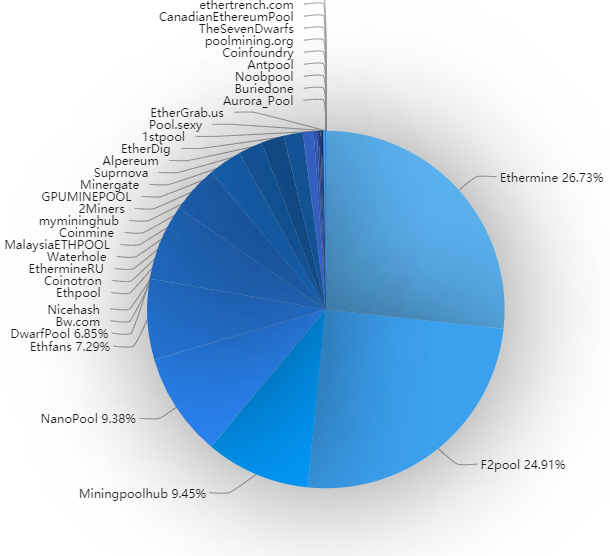
\includegraphics[scale=0.68]{images/ethpools.png}
\caption{Ethereum mining pool distribution in February 2018 \textnormal{\citep{ethminingpools}}.}
\label{fig:etherpools}
\end{figure}

However, the chance of that happening is fractional. I assume that as soon as there would be an evidence of such an act happening, miners would just switch pools, thus reducing the attacking pools' hashrates and, therefore, ending the attack.

When considering DDoS attacks, Ethereum-based applications are highly resistant against those, as it would be too expensive to perform such an act if a smart contract application is implemented properly. Client-server applications' DDoS protection is strongly dependent on migration and traffic filtering tools, that are used to protect the service. This has not been tested in practice during the study.

\paragraph{Encryption}
Encryption was unfortunately not implemented in both applications and left for future work, which is described in Section \ref{section:futurework}. Therefore, different encryption solutions could not be tested and compared between two systems.

\subsubsection{Cost analysis} \label{section:costpractical}

\paragraph{Logistics costs}
Cost is a very important aspect to the users, that are planning to use a service. Cost of using the centralized application can be compared to the original service by Blocket. Pricing of the original service includes shipping with cash-on-delivery \citep{cod} by DBSchenker, management of agreement payments and potential conflict resolving, if necessary. A smaller package, that weighs around 1 kg, costs around 13 USD to transfer using the original system. In case of item being disapproved by the buyer, the buyer himself needs to pay around 10 USD for the return. 

Shipping of the item without using the Secure Package service, comes at a cost of around 10 USD (depending on the logistics company), with the returns, obviously, costing as much as delivery does. The addition of cash-on-delivery comes at a cost of about 14 USD in case of Postnord (DBSchenker does not offer this service to regular packages, however, they have a deal with Blocket). It is clear, that the deal between Blocket and DBSchenker results in quite a large decrease in price for a customer, as the cash-on-delivery service is included into the price, but is only a few dollars more expensive then the regular shipping.

When comparing the two systems, it is important to consider that cash-on-delivery functionality is provided by the smart contract, so users may use regular cheaper shipping to send packages. Thus, the blockchain-based service is about 3 USD cheaper to use from that standpoint, then the centralized implementation.

\paragraph{Sensor inclusion}
When considering sensor inclusion, it is difficult to predict how much that functionality would cost. As described in \ref{section:sensorsupported}, introduction of that service would require massive investments into infrastructure of the logistics process by the companies, thus driving the price up. Nevertheless, regardless of sensor inclusion cost, the pricing of sensors is considered being equal for both systems in context of this cost analysis.


\paragraph{Additional fees}
Usage of the centralized application does not pose any additional costs to the users, besides that overhead, which is included into the shipping cost (thanks to which, the company that runs the service make their profit). That is not the case in the Ethereum-based application, due to the transaction fees, associated with smart contract interaction. Different operations come at different costs for the users, depending on the situation. As shown in Figure \ref{fig:blockchaincost}, the total amount, spent by different actors, increases with addition of more sensors, presence of the return and clerk resolving. This is due to increased number of interactions, which is required by the application. It is important to consider that the cost proportionally increases with increase in gas price.

\pgfplotsset
 {
 /pgfplots/ybar legend/.style={
 /pgfplots/legend image code/.code={
 \draw[##1,/tikz/.cd,yshift=-0.25em]
 (0cm,0cm) rectangle (20pt,0.8em);},
 },
}
\begin{figure}[H]
\centering
\pgfplotstableread{
	%seller			%buyer			%logistics
0   1.8206          0.7754				0.7338
1   2.0590          0.8967				0.8629
2   3.0116          1.3822				1.3749
3	3.3202			1.1926				1.6741				
4	3.4371			1.1926				2.0063
5	4.2464			1.1926				2.0063
}\dataset
\begin{tikzpicture}
\begin{axis}[
    ybar,
    bar width = 0.5cm,
    width=15cm,
    ymin=0,
    ymax=5,
    xtick=data,
    xticklabels =
    {
        \small{Successful(0)},
        \small{Successful(1)},
        \small{Successful(5)},
        \small{Returned(5)},
        \small{Disapproved(5)},
        \small{Resolved(5)}
    },
    xticklabel style={rotate=0},
    major x tick style = {opacity=0},
    minor x tick num = 1,
    minor tick length=2ex,
    every node near coord/.append style={anchor=west, rotate=90},
    legend entries={Seller account, Buyer account, Logistics account},
    legend columns=3,
    legend style={at={(0.5,1)},,anchor=north,draw=none,nodes={inner sep=3pt}},
    ]
  \addplot[draw=black,fill=blue!60, nodes near coords] table[x index=0,y index=1] \dataset; 
  \addplot[draw=black,fill=red!60, nodes near coords] table[x index=0,y index=2] \dataset; 
  \addplot[draw=black,fill=orange!60, nodes near coords] table[x index=0,y index=3] \dataset;
\end{axis}

\end{tikzpicture}
\caption{Cost analysis of additional fees in the blockchain-based application \textnormal{\citep{axelrapport}}. Values within the parenthesis indicate number of sensors attached. Gas price of 3 Gwei was used.}
\label{fig:blockchaincost}
\end{figure}

As mentioned in \ref{section:pracusability}, these additional fees, related to gas price were one of the main reasons why it is not possible to add pictures and descriptions to the agreement in blockchain-based implementation. Apparently, a trade-off in favor of cost-effectiveness was made during the development of decentralized Secure Package.

\paragraph{Total cost}
The total cost of using each service depends on the sum of logistics costs $P_l$, sensor inclusions $P_s$ and additional fees $P_f$, as derived in Equation (\ref{eq:totcost}). 

\begin{equation} \label{eq:totcost}
T = P_l + P_s + P_f
\end{equation}

In order to get bigger picture of the cost analysis, several cases are considered. Sensor inclusion logistics fee is equal for both systems and is denoted by $s$. Total cost of using the centralized application is denoted by $T_c$ and total cost of using the blockchain-based application is denoted by $T_b$.

\begin{itemize}
\item \textbf{Successful agreement (0 sensors)}
\begin{align*}
T_c &= 13 + 0 \cdot s + 0 = 13\\
T_b &= 10 + 0 \cdot s + 3.33 = 13.33
\end{align*}
\item \textbf{Successful agreement (5 sensors)}
\begin{align*}
T_c &= 13 + 5 \cdot s + 0 = 13 + 5s\\
T_b &= 10 + 5 \cdot s + 5.76 = 15.76 + 5s
\end{align*}
\item \textbf{Agreement with an approved return (5 sensors)}
\begin{align*}
T_c &= 13 + 10 + 5 \cdot s + 0 = 23 + 5s\\
T_b &= 2 \cdot 10 + 5 \cdot s + 6.18 = 26.18 + 5s
\end{align*}
\item \textbf{Agreement, in which the conflict occurred and logistics company was liable (5 sensors)}
\begin{align*}
T_c &= 13 + 10 + 5 \cdot s + 0 = 23 + 5s\\
T_b &= 2 \cdot 10 + 5 \cdot s + 7.45 = 27.45 + 5s
\end{align*}
\end{itemize}

By studying the scenarios above, it is clear, that the centralized solution is slightly cheaper. However, for the blockchain-based solution, the gas price of 3 Gwei is chosen, which is good enough in case of moderate congestion. When Ethereum network becomes highly congested, the recommended gas price may drastically increase, thus making the blockchain-based solution a lot more expensive.

\paragraph{Price volatility}
Ether, which is used for payments in the decentralized application is extremely volatile. A possible scenario, which describes the reasoning behind why the usage of centralized system is more beneficial to sellers was described in Section \ref{section:fiatoption}.

\subsubsection{Reusability and modifiability}
Once deployed, the blockchain-based application's main contract resides on a distinct address of the Ethereum network. The application is public and can be accessed by other services by interacting with the main contract, which makes it highly reusable. It is also possible to modify the smart contract code and deploy the application on another address.

In case of the client-server application, the code can also be modified, recompiled and deployed, as it is available to the public in order to increase the transparency. Modular structure of Angular-based applications allows for easy integration of additional modules, which makes it easily modifiable. The API allows for easy integration of the application's backend to other services.

\subsubsection{Environmental effect}
As the client-server application was not deployed on a real server and was only tested locally, its actual power consumption was not tested. Therefore, theoretical analysis on this subject in Section \ref{analysis:environmental} was considered as the main reference. Ethereum is a proof-of-work blockchain and its mining process is extremely power hungry. Deployment of additional DApps on Ethereum has to be supported by presence of additional computational power. As of now, Ethereum draws six times more power than Facebook does. Thus, if the centralized Secure Package was to handle 6 times more requests than Facebook does, it would consume as much power as Ethereum, which, at the time of writing, can handle at most 76200 transactions per hour, as derived from Equation (\ref{eq:eththroughput}). In comparison to Ethereum, Facebook is regularly used by around 2.1 billion people at the time of writing \citep{faceusers}, which generates alot more than Ethereum's maximum transaction density of 76200 transactions per hour.

\subsubsection{Constraints}
In terms of the centralized application, the only real constraints would be the ones that are related to its hardware architecture's performance. However, as discussed before, these constraints can potentially be addressed by simply upgrading the hardware.

In case of the Ethereum-based application, the majority of constraints are related to the cost, associated with smart contract interaction and storage of data. This affected the implementation process, as some trivial functionality was not implemented in order to not make the application too expensive to use. An example of such functionality is sensor data visualization. The centralized system stores all of the sensor data, in order to be able to display it to the users, if so desired. This is not the case in the decentralized implementation of the system, in which only violation events are stored, as it is alot more cost-effective. In other words, a trade-off between cost-effectiveness and usability was made in favor of the first one. 

Latency is another constraint in the blockchain-based application, as there is no way of telling when the data will be added to the chain.

\subsubsection{Usability} \label{section:pracusability}

\paragraph{Marketplace functionality}
It is extremely expensive to store data in Ethereum. By looking at Table \ref{tab:imgdescscenarios}, we can see that it costs approximately 184 USD$^\star$ to store two pictures and a 100 character long description in Ethereum. That is one of the reasons, why the web marketplace functionality was not implemented as part of the blockchain-based system, as it would simply be too expensive for users to create advertisements for their items. Therefore, the system focuses mainly on the payments and transport of the item.

The centralized application, however, is not constrained in that aspect. MySQL database can handle enormous amounts of data at no additional cost, thus making addition of high resolution images and long descriptions accessible to the users. Therefore, a fully functional all-in-one web marketplace could be implemented.

\paragraph{Responsiveness}
The centralized application is responsive, as communication with a MySQL database backend via an API is done very quickly and efficiently. When comparing the responsiveness aspect of two systems, the centralized application is a clear winner, as there is next to no latency, which could not be said about the decentralized Ethereum-based application. The reason for that is the unpredictable block confirmation delay, which was discussed in Section \ref{section:performancepractical}.